\chapter{Výsledky a diskuse}
Kapitola shrnuje a interpretuje výsledky parametrizací metod EEM a PEOE za užití navržených klasifikací atomů s cílem zhodnotit, zda jsou pro parametrizaci vhodné detailní klasifikace atomů či pro tento problém postačují základní hrubá dělení. Veškeré výstupy parametrizací lze nalézt v externí příloze bakalářské práce nebo na webové adrese \url{https://lcc.ncbr.muni.cz/~raduse19/}.  

\section{Vstupní data}
Pro parametrizaci empirických metod byla použita molekulová sada CCD\_gen a sada Protein (viz tab. \ref{moleculesets}). Pro analýzu přenositelnosti parametrů byly molekuly v molekulových sadách rozděleny na sadu tréninkovou a validační v poměru 9:1. Software MACH zajistil, aby validační sada vždy obsahovala identické atomové typy jako sada tréninková. Empirické metody byly pro obě molekulové sady parametrizovány vůči referenčním nábojům typu B3LYP/6-311G*/NPA.
% Klasifikace určené pro formát SDF byly nejdříve zkušebně aplikovány na tréninkovou sadu obsahující 500 molekul a použity pro parametrizaci. 
\begin{table}[h]
    \renewcommand{\arraystretch}{1.35}
    \centering
    \begin{tabular}{l|l|l}
         sada molekul &  \textbf{CCD\_gen} \cite{krab1k}
         & \textbf{Protein}\\
         \hline
         počet molekul & 4 443 & 32\\
         počet atomů & 204 760 & 29 107\\
         počet atomů v molekule & 3–305 & 166–1 174 \\
         zdroj struktur & software CORINA & RTG krystalografie \\
         \hline
         \multirow{2}{8em}{molekuly} & 
            ligandy z databáze PDB & malé proteiny\\
         & pouze validní struktury & \makecell[l]{neobsahují ligandy ani \\nestandardní residua}
    \end{tabular}
    \caption{Souhrn informací o molekulových sadách užitých pro parametrizaci. Molekuly obou sad 
    byly doplněny o atomy vodíku a byla optimalizována jejich geometrie.}
    \label{moleculesets}
\end{table}

% \makecell[l]{malé proteiny bez ligandů\\a nestandarních residuí}\\
\section{Výsledky parametrizace}
Pro popis výsledků parametrizací empirických metod za užití různých klasifikátorů je zavedeno značení 'molekulová sada/empirická metoda/užitý klasifikátor'. Výpočty  parametrizací probíhaly na serverech virtuální organizace MetaCentrum. 

Implementované klasifikátory jsou srovnány s triviální referenční klasifikací \verb|plain|, která rozděluje atomy do atomových typů na základě hodnoty protonového čísla. 
%markantní rozdíly byly nalezeny zejména v čase výpočtu jednotlivých parametrizací.
%Výsledky všech parametrizací používajících implementované klasifikátory jsou srovnávány s referenčním klasifikátorem \verb|plain|, který dělí atomy do atomových typů dle  protonového čísla.
%Pro každý klasifikátor je výsledek dané parametrizace srovnán s parametrizací využívající klasifikaci atomů dle protonového čísla. 
%Referenční klasifikátor, označen jako \verb|plain|, je implementován v softwaru MACH. 
Klasifikátor \verb|partners| generuje pro obsáhlé molekulové sady extrémní množství atomových typů (pro sadu CCD\_gen konkrétně 235%, tzn. téměř 500 hledaných parametrů pro metodu EEM
), jeho použití proto nelze obecně doporučit. 

Hodnota PCC$^2$ napříč parametrizacemi za užití obou molekulových sad neklesá pod hodnotu 0,97; lze tedy vyvodit, že náboje atomů získané skrze vypočtené parametry silně lineárně korelují s referenčními náboji (viz obr. \ref{graph_corr_EEM}). Hodnoty RMSD  pro vypočtené empirické a~referenční náboje (dále jen 'hodnoty RMSD') se pohybují nejčastěji v rozmezí 0,040-0,060; u PDB sady v některých případech klesají až k hodnotě 0,023. Uvedená rozmezí hodnot statistik platí jak pro tréninkové, tak validační sady molekul. Statistiky parametrizací sady CCD\_gen lze nalézt v následující tabulce \ref{statistics}. Statistiky parametrizací sady Protein jsou umístěny v~příloze \ref{proteinstat}. 
\medskip
\begin{table}[h]
    \small
    \renewcommand{\arraystretch}{1.4}
    \centering
    \begin{tabular}{l|l|l|l|l|l|l|l}
         \textbf{klasifikátor} & \textbf{\textit{n}} & \textbf{metoda} & \textbf{RMSD} & \textbf{PCC$^2$} & \textbf{MAE} & \textbf{ABSMAX} & \textbf{doba výpočtu}\\
         \hline
         \multirow{2}{6em}{\texttt{plain}} & \multirow{2}{1.5em}{ 9} & EEM & 0,0641 & 0,9768 & 0,0440 & 0,7455 & 1:01:08 \\
         & & PEOE & 0,0516 & 0,9849 & 0,0343 & 0,5228 & 0:55:06 \\
         \hline
         \multirow{2}{6em}{\texttt{hbo}} & \multirow{2}{1.5em}{19} & EEM & 0,0582 & 0,9809 & 0,0405 & 0,7133 & 1:59:29  \\
         & & PEOE & 0,0394 & 0,9912 & 0,0259 & 0,7313 & 2:53:04 \\
         \hline
         \multirow{2}{6em}{\texttt{hybrid}} & \multirow{2}{1.5em}{15} & EEM & 0,0620 & 0,9781 & 0,0424 & 0,7475 & 1:15:40 \\
         & & PEOE & 0,0479 & 0,9870 & 0,0310 & 1,0619 & 1:42:28 \\
         \hline
         \multirow{2}{6em}{\texttt{substruct}} & \multirow{2}{1.5em}{64} & EEM & 0,0479 & 0,9870 & 0,0300 & 0,6593 & 17:46:49 \\
         & & PEOE & 0,0464 & 0,9878 & 0,0293 & 0,9175 & 6:56:11 
    \end{tabular}
    \caption{Výsledky vybraných statistik parametrizace CCD\_gen sady, \textit{n} značí počet užitých atomových typů. Jsou zaznamenány pouze statistiky tréninkových sad.}
    \label{statistics}
\end{table}
\medskip
 
PCC$^2$ získaných empirických a referenčních nábojů nabývá napříč parametrizacemi minimální hodnoty 0,9768 pro CCD\_gen/EEM/plain parametrizaci, hodnota RMSD je maximálně 0,0641, a to u téže parametrizace. Ve srovnání s implementovanými klasifikacemi jsou parametrizace za užití klasifikátoru \verb|plain| méně časově náročné. Hodnoty RMSD pohybující se kolem hodnoty 0,060 patří napříč parametrizacemi k nejvyšším, hodnoty PCC$^2$ empirických a referečních nábojů se jsou u klasifikace \verb|plain| vůči implementovaným klasifikátorům snížené v řádu tisícin, výjimečně setin. 

Rozdíl hodnot RMSD tréninkových a validačních sad je napříč parametrizacemi nejčastěji v řádu desetitisícin, maximální hodnota tohoto rozdílu je 0,018. Hodnoty PCC$^2$ zmíněných sad se liší v~řádu tisícin či desetitisícin, pro MAE a ABSMAX rozdíl proniká až do řádu setin. Na základě těchto údajů lze  parametry získané užitím implementovaných klasifikátorů pokládat za přenositelné. Hodnoty statistik tréninkové a validační sady klasifikátoru \verb|hbo| ilustruje tabulka \ref{prenositelnost} níže.

\begin{table}[h]
    \renewcommand{\arraystretch}{1.4}
    \centering
    \begin{tabular}{c|l|l|l|l|l}
         \textbf{metoda} & \textbf{sada} & \textbf{RMSD} & \textbf{PCC$^2$} & \textbf{MAE} & \textbf{ABSMAX}\\
         \hline
         \multirow{2}{4em}{EEM} & train & 0,0582 & 0,9809 & 0.0405 & 0,7133  \\
         & test & 0,0566 & 0,9819 & 0,0397 & 0,7045 \\
         \hline
         \multirow{2}{4em}{PEOE} & train & 0,0394 & 0,9912 & 0.0259 & 0,7313  \\
         & test & 0,0386  & 0,9916 & 0,0258 & 0,4765 \\
    \end{tabular}
    \caption{Porovnání statistik parametrizací CCD\_gen/EEM(PEOE)/hbo. Statistiky tréninkových a validačních sad vykazují minimální rozdíly.}
    \label{prenositelnost}
\end{table}

\begin{figure}[H]
\begin{center}
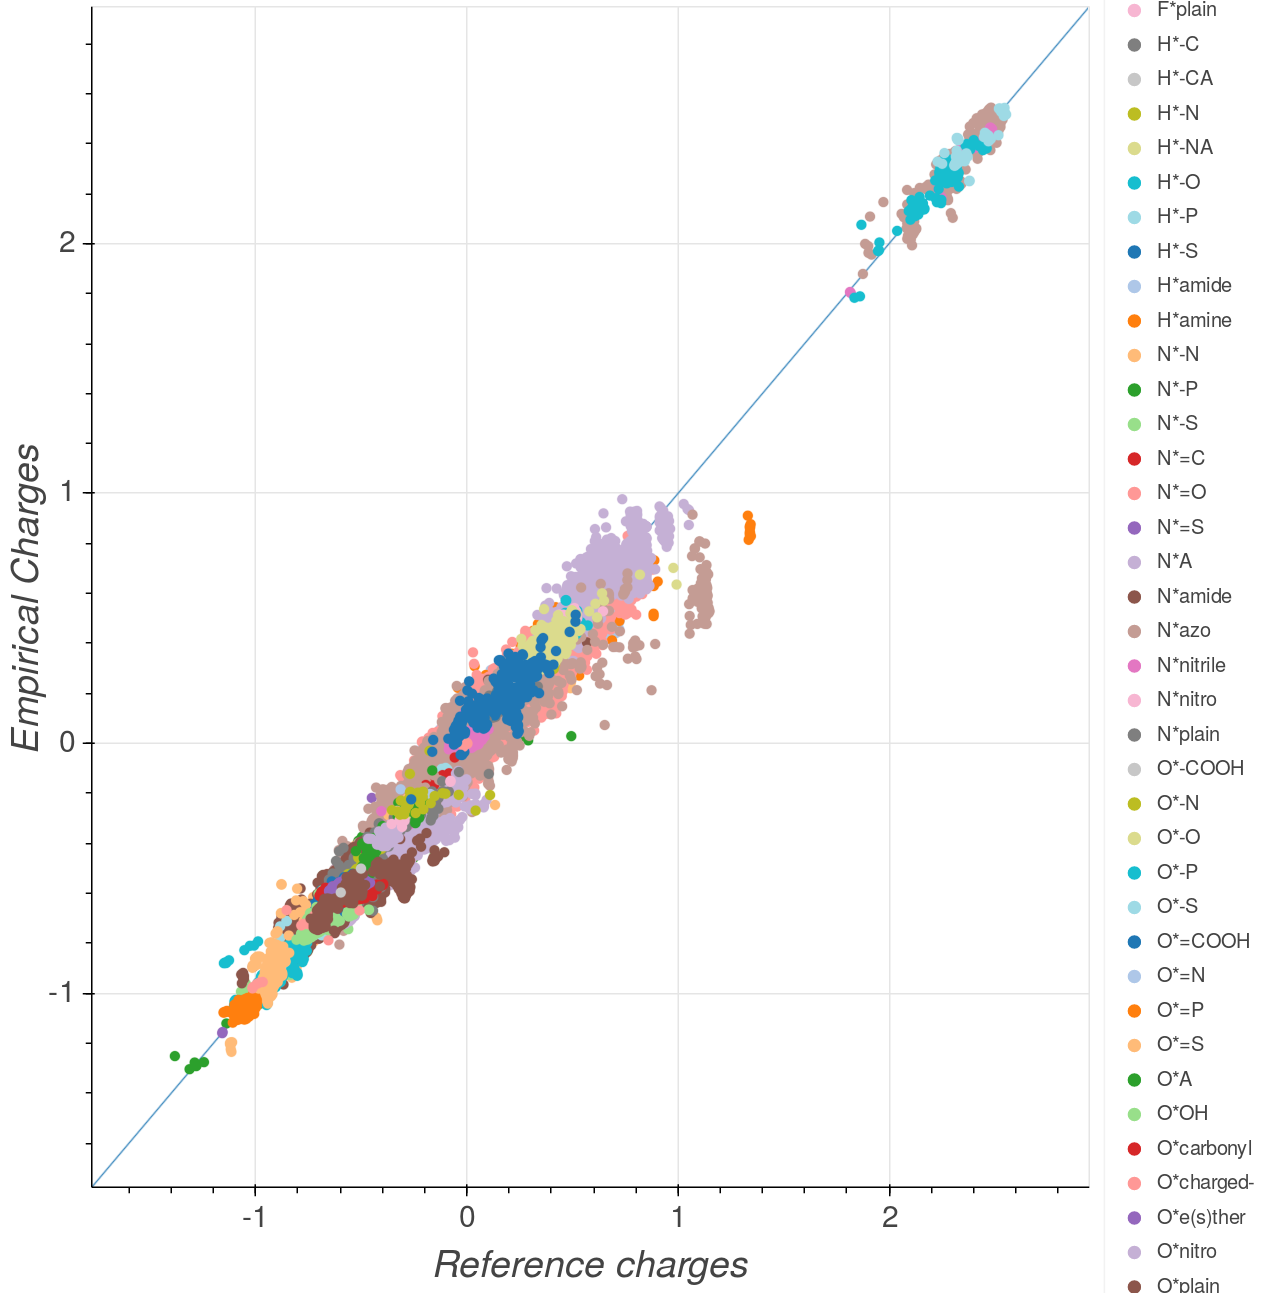
\includegraphics[width=13cm]{pictures/graph_correlation_SDF_EEM_substruct.png}
\caption{Korelační graf parametrizace CCD\_gen/EEM/substruct.  PCC$^2$=0,9870; RMSD=0,0479. Legenda ve skutečnosti obsahuje 64 atomových typů, v obrázku je oříznuta na~velikost grafu.}
\label{graph_corr_EEM}
\end{center}
\end{figure}
\newpage

Z korelačních grafů empirických a referenčních nábojů je patrné, že metoda PEOE přiřazuje v určitých případech atomům náboje o konstatní hodnotě, což v grafu odpovídá vodorovným shlukům bodů (viz obr. \ref{graph_corr_PEOE} nebo obr. \ref{graph_peptidesimpl_PEOE} v příloze). Přiřazení konstaních či velmi podobných hodnot parciálních nábojů vyplývá z iterativního způsobu výpočtu. Atomu je iniciálně přiřazena hodnota jeho formálního náboje. V každé iteraci výpočtu dochází k přesunu elektronové hustoty mezi vazebnými partnery, přičemž se toto množství exponenciálně snižuje, a to až do ustálení výsledné hodnoty parciálního náboje. Metoda PEOE navíc pracuje pouze s~topologií molekuly a atomům, které mají stejné chemické okolí, implicitně přiřazuje stejné náboje.

\vspace*{1cm}
\begin{figure}[H]
\begin{center}
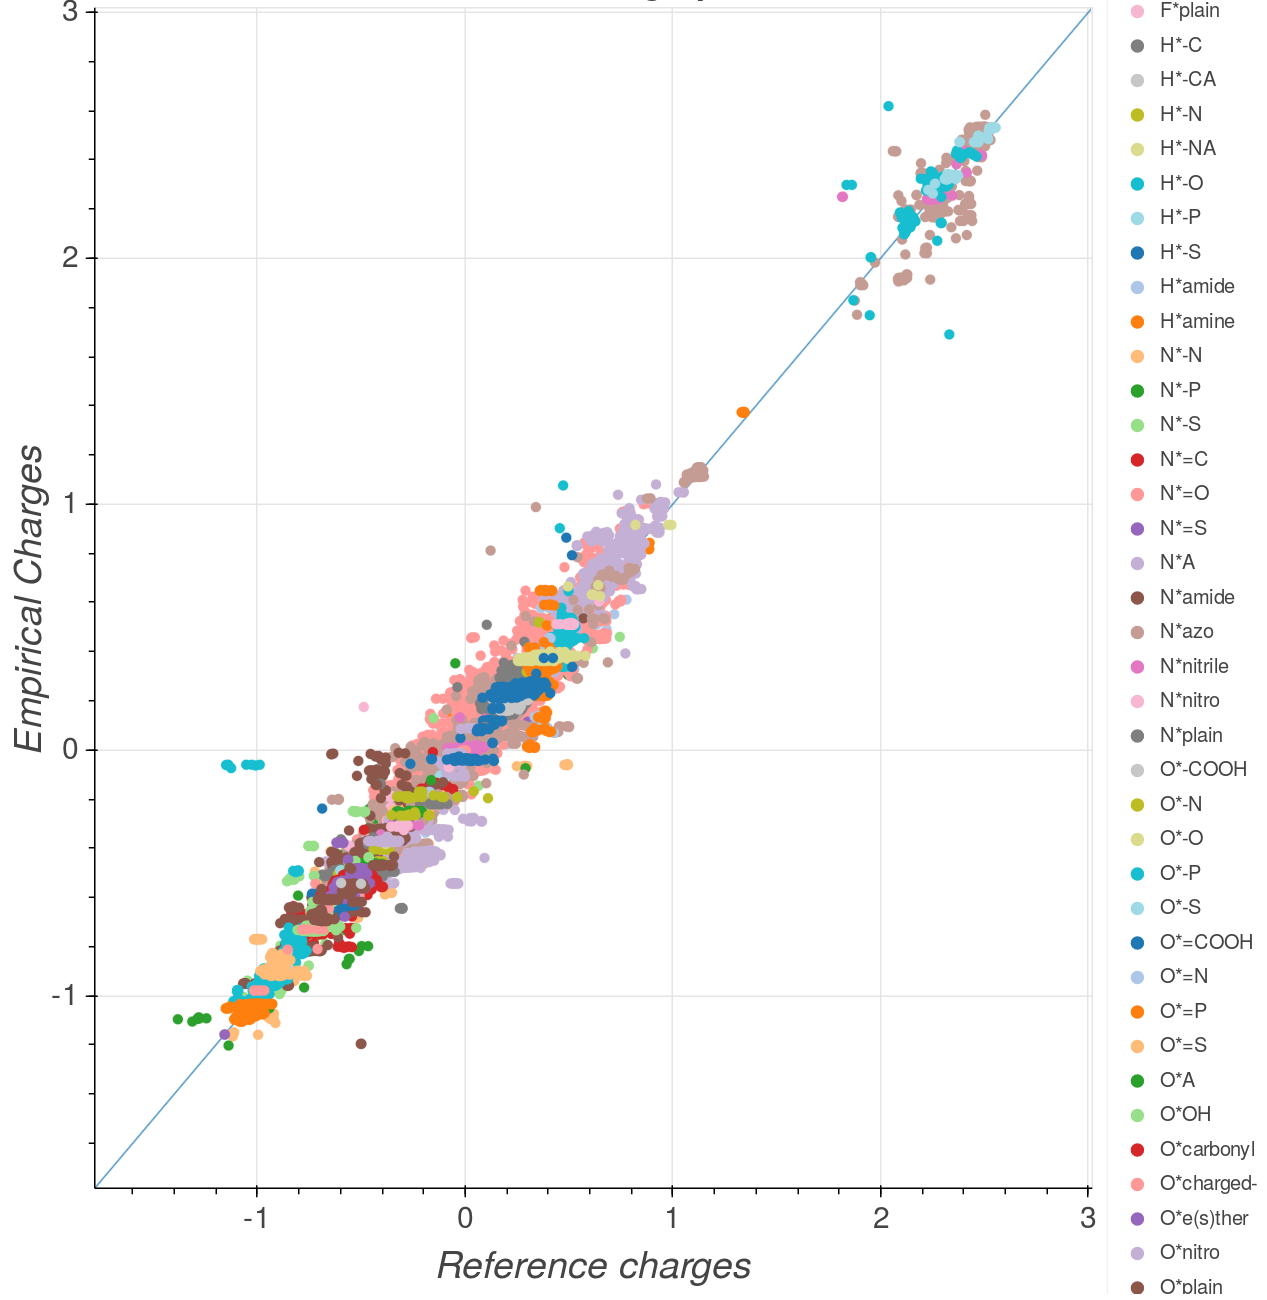
\includegraphics[width=14cm]{pictures/graph_PEOE_substruct.png}
\caption{Korelační graf parametrizace CCD\_gen/PEOE/substruct.  PCC$^2$=0,9878; RMSD=0,0464. Legenda ve skutečnosti obsahuje 64 atomových typů, v obrázku je oříznuta na~velikost grafu.}
\label{graph_corr_PEOE}
\end{center}
\end{figure}

\subsection{Úprava klasifikátorů 'substruct' a 'peptide'}
Časová náročnost parametrizací za použití klasifikátorů \verb|substruct| a \verb|peptide| se v porovnání s ostatními klasifikátory ukázala jako netriviální z důvodu velkého množství definovaných atomových typů. Po analýze korelačních grafů byly vybrané atomové typy sloučeny, nejčastěji na základě nejvyššího řádu vazby daného atomu (atomové typy popisující jednovaznou síru navázanou na dusík, fosfor a síru byly sloučeny pod atomový typ 'S*1bond'), v případě vodíků byly sloučeny atomové typy popisující vodíky navázané na atomy o stejném protonovém čísle. Počet atomových typů byl u obou klasifikátorů zredukován přibližně na polovinu. Korelační grafy parametrizací za užití redukovaného klasifikátoru \verb|peptide| jsou zobrazeny v příloze \ref{priloha_peptide}.

\begin{table}[h]
    \renewcommand{\arraystretch}{1.4}
    \centering
    \begin{tabular}{c|l|l|l|l|l|l}
         \textbf{klasifikátor} &  \textbf{metoda} & \textbf{RMSD} & \textbf{PCC$^2$} & \textbf{MAE} & \textbf{ABSMAX} & \textbf{doba výpočtu}\\
         \hline
         \multirow{2}{6em}{\texttt{substruct}} & EEM & 0,0334 & 0,9948 & 0,0229 & 0,3880 & 23:01:14  \\
         & PEOE & 0,0493 & 0,9887 & 0,0292 & 0,4484 & 0:19:51 \\
         \hline
         \multirow{2}{6em}{\texttt{substruct simplified}} & EEM & 0,0388 & 0,9930 & 0,0265 & 0,3198 & 14:30:45 \\
         & PEOE & 0,0514 & 0,9876 & 0,0319 & 0,5083 & 0:13:02 \\
         \hline
         \multirow{2}{6em}{\texttt{peptide}} & EEM & 0,0359 & 0,9940 & 0,0228 & 0,3558 & 1 den, 15:03:35 \\
         & PEOE & 0,0456 & 0,9902 & 0,0293 & 0,3147 & 0:29:01 \\
         \hline
         \multirow{2}{6em}{\texttt{peptide simplified}} & EEM & 0,0389 & 0,9929 & 0,0266 & 0,3647 & 18:28:26 \\
         & PEOE & 0,0512 & 0,9877 & 0,0302 & 0,2536 & 0:15:12
    \end{tabular}
    \caption{Srovnání statistik původních a zjednodušených klasifikátorů \texttt{peptide} a~\texttt{substruct} aplikovaných na sadě Protein. V tabulce jsou zaznamenány pouze statistiky tréninkových sad.}
    \label{statistics_simplified}
\end{table}

Statistiky zjednodušených klasifikací se od statistik původních klasifikátorů liší pou\-ze minimálně, rozdíly hodnot jednotlivých statistik se týkají řádu tisícin, ve výjimečných případech setin. Zjednodušením klasifikace se docílilo snížení časové náročnosti parametrizace zhruba na polovinu, a to s minimálním vlivem na kvalitu vypočtených parametrů.

%Výsledky redukce atomových typů klasifikátorů \verb|substruct| a \verb|peptide| potvrdily hypotézu, že klasifikace atomů s menším množstvím definovaných atomových typů jsou pro účely parametrizace z výpočetního hlediska vhodnější než detailní klasifikace, přičemž statistiky empirických a referenčních nábojů zůstávají při zavedení méně detailních klasifikací oproti podrobným klasifikacím téměř nezměněny.

\subsection{Statistiky vybraných atomových typů}
Vysoká hodnota PCC$^2$ molekulové sady popisuje míru lineární závislosti hodnot empirických a referenčních nábojů, nevypovídá však o lineární korelaci mezi empirickými a~referenčními náboji pro jednotlivé atomové typy.

Pro vybrané atomové typy nabývá PCC$^2$ hodnot blízkých nule, mezi atomy, které jsou daným atomovým typem klasifikované, je tedy detekována nulová lineární závisost mezi empirickými a referenčními náboji. Nízká hodnota kvadrátu Pearsonova korelačního koeficientu vybraného atomového typu může být způsobená přiřazenou konstantní hodnotou empirických nábojů nebo malým počtem atomů, který atomový typ reprezentují. I minimální odchylky nábojů od přímky $y = x$ korelačního grafu se projeví do výsledné hodnoty PCC$^2$ atomového typu, zejména v případě, kdy je rozsah hodnot referenčních nábojů  velmi malý. 

Nízká hodnota PCC$^2$ atomového typu nepředstavuje problém, pokud se hodnoty empirických a referenčních nábojů liší pouze minimálně. Uvedené tvrzení platí pro atomové typy 'H*C', 'O*carbonyl' a 'O*OH' v obr. \ref{graph_pcc_atom_types}. Statistiky vybraných atomových typů lze nalézt v [příloze]. 


\vspace{0,5cm}
\begin{figure}[h]
\begin{center}
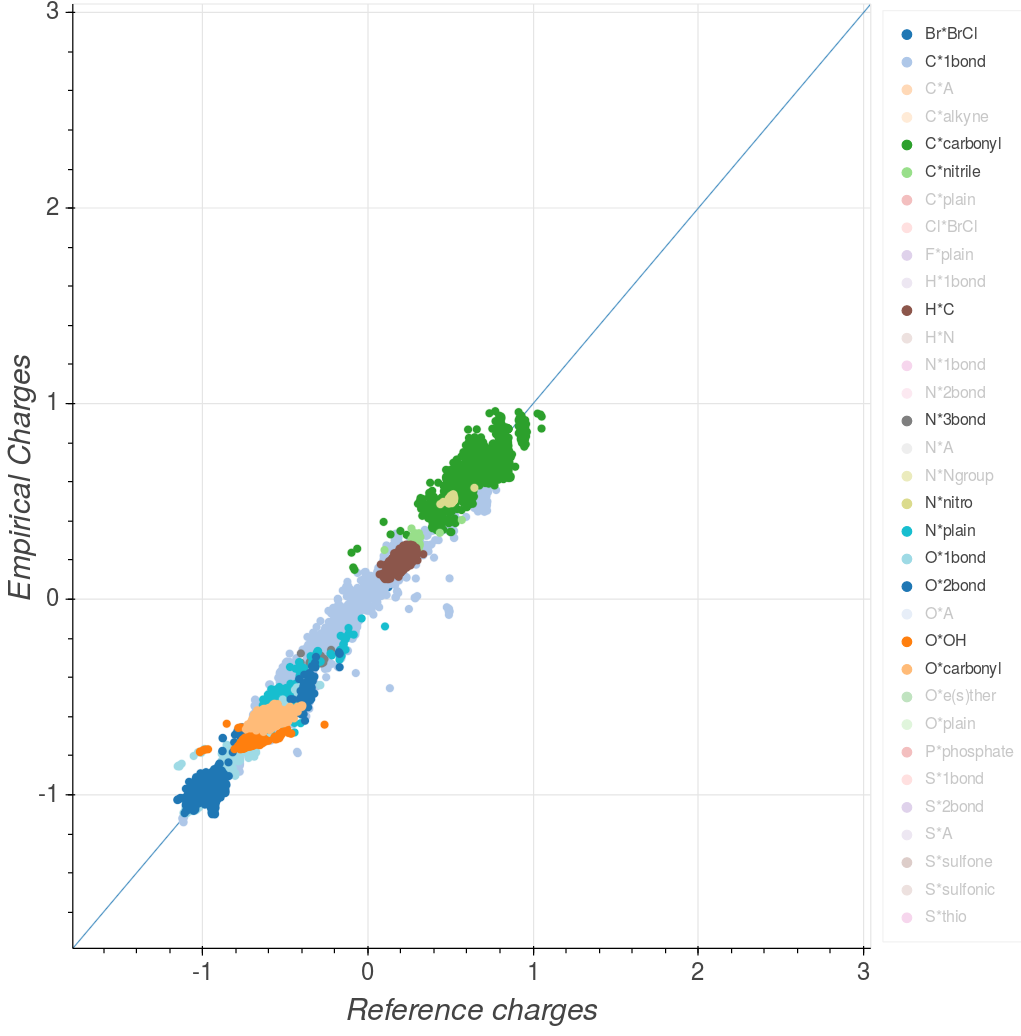
\includegraphics[width=13cm]{pictures/graph_pcc_atom_types.png}
\caption{Korelační graf parametrizace CCD\_gen/EEM/substruct\_simplified. PCC$^2$ pro atomové typy 'H*C', 'O*carbonyl' a 'O*OH' nabývá hodnot 0,3702; 0,1501 a 0,3050.}
\label{graph_pcc_atom_types}
\end{center}
\end{figure}

\noindent Ze šesti klasifikátorů implementovaných v knihovně ATTYC se pět klasifikací atomů prokázalo platnými pro parametrizaci empirických metod EEM a PEOE. Nezanedbatelné rozdíly byly napříč klasifikátory nalezeny pouze v době výpočtu jednotlivých parametrizací. Analýza parametrizací za užití implementovaných klasifikátorů ve srovnání s referenční klasifikací prokázala, že základní klasifikace atomů využívající malý počet atomových typů jsou pro potřeby parametrizace plně dostačující.
% Hodnota PCC$^2$ atomového typu 'C*1bond' je 0,9316.

% \begin{figure}[h]
% \begin{center}
% 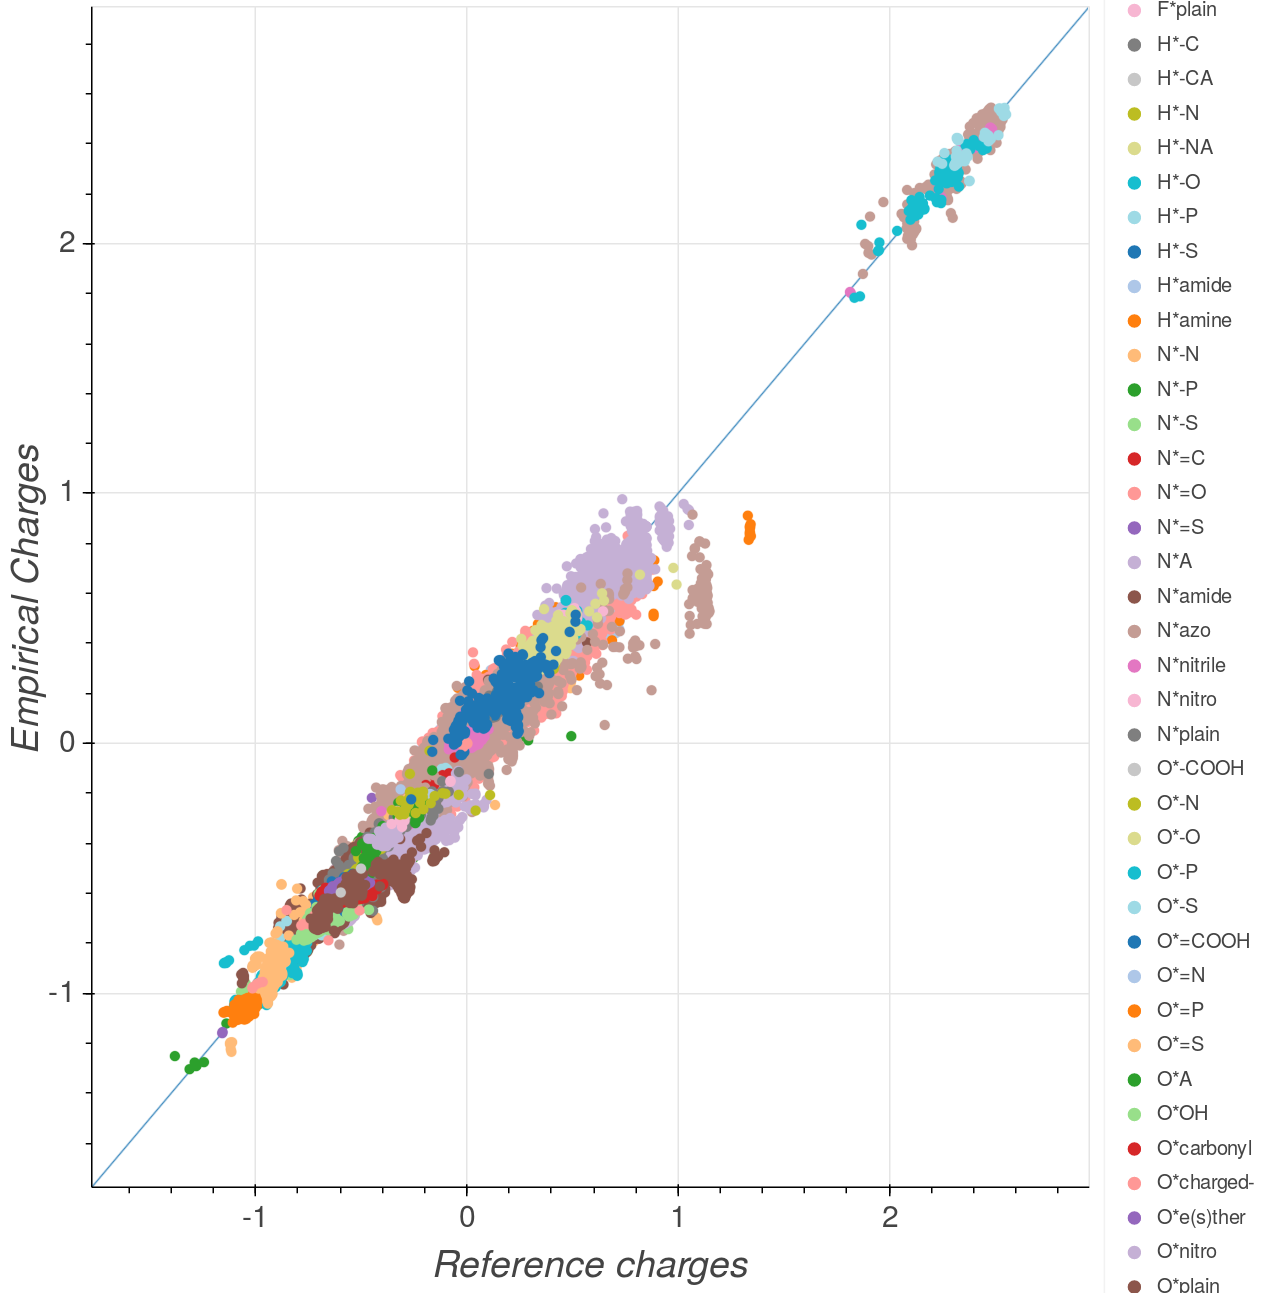
\includegraphics[width=14cm]    {pictures/graph_correlation_SDF_EEM_substruct.png}
% \caption{Korelační graf parametrizace SDF/EEM/substruct.  PCC$^2$=0,9870; RMSD=0,0479. Legenda ve skutečnosti obsahuje 64 atomových typů, v obrázku je oříznuta na~velikost grafu.}
% \label{graph_corr}
% \end{center}
% \end{figure}